\chapter{Methodology}

\section*{from workplan}
etc

\section{Identification of signal points}
Most of the studies that try to find bathymetric points from Icesat-2 use some variation of the DBSCAN algorithm to identify possible bathymetric signal. The algorithm has the advantages of being robust to noise \cite{} and very computationally efficient. However, one disadvantage is that is is very sensitive to the choice of parameter values, and setting them programatically so that they work on a global scale basis is difficult \cite{}.

\subsection{Filter to subsurface photons}
The raw photon cloud from the ATL03 data product contains many photons from land, clouds, the sea surface, and noise. Before applying an algorithm to extract bathymetric signal from noise, first areas of the photon cloud that could not contain bathymetric signal must be removed. A filtering algorithm was developed to cull points in the following steps:

\begin{enumerate}
    \item For each point, extract the elevation from the GEBCO dataset. Any points have a GEBCO elevation value of greater than +6m or less than -50m are removed. It is assumed that any points with a GEBCO elevation greater than 6 meters can be reliably assumed to be land, and any points with an elevation less than -50 can be reliably assumed to be noise. This is based on the maximum depth that ICESat-2 has been demonstrated to be able to see, as found by \cite{Parrish2019}. This removes points horizontally from areas that are not likely to contain bathymetric signal
    
    \item Cull any points 5m above the geoid

    \item Calculate the sea surface for each point. This can be done using the rolling median of the remaining points with window width n=?\todo{fill in and justify value} of points that are marked as high confidence ocean signal \parencite{Ranndal2021}. Then subtract the Z elevation to get the depth below the ocean surface.  Cull any points deeper than 40m. This provides the vertical filtering. 
    \item Cull any points within a buffer distance of the sea surface. This removes the strong signal associated with the sea surface.
\end{enumerate}

After applying the filtering steps above, the remaining points are then evaluated for bathymetric signal. Several methods common methods in the literature explained in section \ref{subsec:denoising}. For this project\todo{reword?}, a new method is proposed:


\begin{enumerate}
    \item apply a window function that finds the kernel density of the subsurface points in the vertical direction. The vertical location of the peak of the kernel density is calculated, as in figure \ref{fig:kdefunc}
    \item If the peak of the kernel density is above a threshold, return the Z elevation of the peak. This is assumed to be the seafloor elevation.
\end{enumerate}

\begin{figure}[htbp]
    \centering
    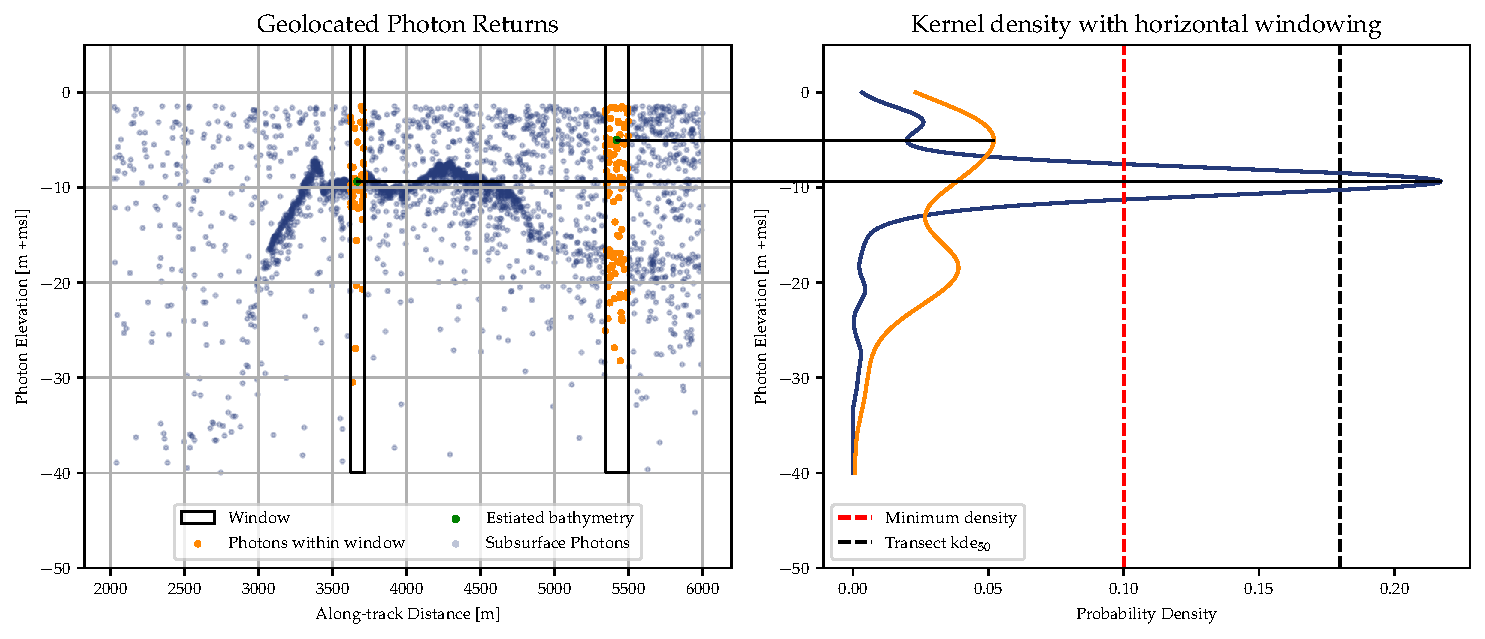
\includegraphics[width=\textwidth]{figures/2d_kde_plot.png}
    \caption{Rolling KDE function applied to photon elevations}
    \label{fig:kdefunc}
\end{figure}

\section{Selection of Test Sites}
\section{Creation of global analysis sites layer}
\subsubsection*{temp notes}

may 25 - what did I do today:
- rewrote testing notebook to use the updated kde seafloor function, and to include some plots showing the trends in the error (ie. error vs depth, error vs kde value, etc)
- Generated the error for florida, and tried to figure out why it was happening. The error is highly concentrated on a few granules from a certain day - it may be clouds on that day.
- if I look at these transects and see what is going wrong, I might be able to find a way to adapt the algorithm to deal with it.

may 31 -

My current method culls points within a buffer of the sea surface, so it struggles to find signal in very shallow (2-3m) water depth. Maybe A-DRAGANN as implemented in \cite{Cao2021} might be more reliable in shallow water?
\todo{temp notes}
\begin{enumerate}
    \color{orange}
    \item Start with 2021 OSM coastline
    \item 
    \item clip to extent of mangroves worldwide - only the tropics and subtropics
    \item project in pseudo mercator
    \item split the lines into 100km segments
    \item select these segments where they touch a mangrove 
\end{enumerate}


\section{Processing of Lidar Data}

\section{Gridding of data}
\subsection{temp notes}
Still need to figure out Kalman filter, but based on the current plan one approach might be...
\begin{itemize}
    \color{orange}
    \item download the xyz data that the gebco data is based on
    \item download and filter photon locations
    \item correct for tide to put them in MSL
    \item Use the pygmt gridding using the xyz data
    \item how to use satellite gravimetry data in gebco? Need to sort that out. Most the MBES data that gebco is based on is available, but the gravimetric seemingly is not.
    \item Decide on what horizontal resolution should be the end goal - choose one or assign dynamically based on available data. 
    \item 
\end{itemize}